\documentclass{beamer}

\usepackage{pgf}  
\usepackage{tikz}
\usetikzlibrary{arrows}
\usepgflibrary{shapes.arrows} 
\usetikzlibrary{intersections}
\usetikzlibrary{calc}
\usetikzlibrary{fit}
\usetikzlibrary{automata,positioning}
\usepackage{pgfplots,stackengine}
\usepackage{fontspec}
\usepackage{fancyvrb}
\usepackage{wasysym}
\usepackage{unicode-math}
\usepackage{import}
\usepackage{rotating}
\usepackage{gensymb}
\usepackage{chemfig}
\usepackage{rotating}
\usepackage{booktabs}
\usepackage{pifont}
\usepackage{wrapfig}
\usepackage{mathtools}
\usepackage{graphbox}
\usepackage{epigraph}
\usepackage{listings}
\usepackage{verbatim}
\usepackage{hologo}
\usepackage[absolute,overlay]{textpos}
\usepackage[euler-digits,euler-hat-accent]{eulervm}
%\logo{\pgfputat{\pgfxy(.45,.5)}{\pgfbox[center]{
\includegraphics[width=1.7cm]{Figures/uu_shadow.pngu}}}}

\usetheme{Copenhagen}
\usecolortheme{beaver}

\definecolor{uured}{RGB}{153,0,0}
\setbeamercolor{block title}{use=structure,fg=white,bg=uured}
\setbeamercolor*{item}{fg=red}

\newcommand{\unilogo}{
  \setlength{\TPHorizModule}{1pt}
  \setlength{\TPVertModule}{1pt}
  \begin{textblock}{1}(26,-10)
   
\includegraphics[height=70pt, align=c]{Figures/uu_shadow.png}
  \end{textblock}
  } 

\pgfmathdeclarefunction{gauss}{2}{%
  \pgfmathparse{1/(#2*sqrt(2*pi))*exp(-((x-#1)^2)/(2*#2^2))}%
}
  
\makeatletter
    \newcases{mycases}{\quad}{%
        \hfil$\m@th\displaystyle{##}$}{$\m@th\displaystyle{##}$\hfil}{\lbrace}{.}
\makeatother

\addtobeamertemplate{frametitle}{}{%
    \unilogo
}
\setlength{\fboxsep}{0pt}

\begin{document}
\graphicspath{{Figures/}}
\setsansfont[ItalicFont = Optima Italic,
             BoldFont = Optima Bold,
             Ligatures=TeX ]
            {Optima Regular}
\setmainfont[ItalicFont = Optima Italic,
             BoldFont = Optima Bold,
             Ligatures=TeX]
            {Optima Regular}
\newfontfamily\commentfont[]{Chalkboard}
\newfontfamily\DejaSans{DejaVuSans.ttf}
\newfontfamily\herculanum[]{Herculanum}
\newfontfamily\timesfont[ItalicFont = Times New Roman Italic]{Times New Roman}
\newcommand{\lmr}{\fontfamily{lmr}\selectfont}
\newfontfamily\zA[Ligatures={Common, Rare}, Variant=1] {Zapfino}
\newfontfamily\zB[Ligatures={Common, Rare}, Variant=2] {Zapfino}
\newfontfamily\zC[Ligatures={Common, Rare}, Variant=3] {Zapfino}
\newfontfamily\zD[Ligatures={Common, Rare}, Variant=4] {Zapfino}
\newfontfamily\zE[Ligatures={Common, Rare}, Variant=5] {Zapfino}
\newfontfamily\zF[Ligatures={Common, Rare}, Variant=6] {Zapfino}
\newfontfamily\zG[Ligatures={Common, Rare}, Variant=7] {Zapfino}
\renewcommand\UrlFont{\color{blue}}
\renewcommand\thefootnote{\textcolor{uured}{\arabic{footnote}}}
\lstset{language=Tex, basicstyle=\ttfamily\scriptsize, frame=single }

\title{{\lmr \LaTeX}}   
\author{Jonathan Alvarsson} 
%\titlegraphic{\vfill\includegraphics[width=18em]{Figures/ORN_large.png}}
\date{April 2020} 

\setbeamertemplate{background}{%
    \parbox[c][\paperheight]{\paperwidth}{%
        \vfill
        \hfill
        
\includegraphics[height=0.65\textheight]{Figures/sigill.png}
    }   
}
\begin{frame}[plain]
\unilogo\titlepage
\begin{tikzpicture}[remember picture,overlay]
\tikz[remember picture, overlay] \fill[uured] (current page.north west) rectangle ++(\paperwidth,-0.5cm);
\end{tikzpicture}%
\end{frame}

\setbeamertemplate{background}{}
\renewcommand{\unilogo}{
  \setlength{\TPHorizModule}{1pt}
  \setlength{\TPVertModule}{1pt}
  \begin{textblock}{1}(0,0)
   
\includegraphics[height=27pt, align=c]{Figures/uu.png}
  \end{textblock}
  } 
\section{Background}
    \begin{frame}
    \frametitle{Outline}
    \begin{minipage}{0.25\textwidth}
    \mbox{}
    \end{minipage}
    \begin{minipage}{0.6\textwidth}
    \tableofcontents[hideallsubsections]
    \end{minipage}
    \end{frame}
    \subsection{What is {\lmr \LaTeX}?}
    \begin{frame}
        \frametitle{Background}
        \framesubtitle{What is {\lmr \LaTeX}?}
        \begin{block}{{\lmr \LaTeX} and {\lmr \TeX}}
        {\lmr \LaTeX} is a \alert{document preparation system} based on the
        {\lmr \TeX} typesetting system. {\lmr \TeX} was written by Donald Knuth
        roughly between the years 1977 and 1989. {\lmr \LaTeX}
        was created in the early 1980s by Leslie Lamport.
        \end{block}
    \end{frame}
    \begin{frame}[fragile]
        \frametitle{Background}
        \framesubtitle{What is {\lmr \LaTeX}?}
            An example:
\begin{lstlisting}
\documentclass{article}
\begin{document}
    \section*{Part 1}
        A small example. \LaTeX\ is often used for math:
        \begin{equation}
            y = \frac{1}{x}
        \end{equation}
    \section*{Part 2}
\end{document}
\end{lstlisting}
        \begin{center}
        \fbox{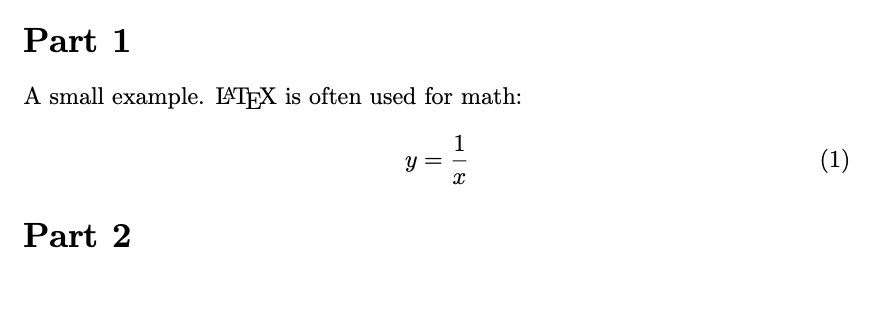
\includegraphics[width=0.5\textwidth]{figures/formath.png}}
        \end{center}
    \end{frame}

    \subsection{Use cases}
    \begin{frame}
        \frametitle{Use cases}
        \framesubtitle{What do I use it for?}
        \begin{block}{What do I use {\lmr \TeX} for?}
            \uncover<2->{(almost)} everything!
            \uncover<3>{
                \begin{itemize}
                    \item This presentation\footnotemark\ is made using it
                    \item When we publish we try to use it
                    \item When I make course materials I use it
                    \item The course book I spend so much time on is made using it
                \end{itemize}
            }
        \end{block}
        \alt<3>{\footnotetext{\mbox{The source code is available at: \url{https://github.com/jonalv/LaTeX_Zoom_presentation_2020}}}}{}
    \end{frame}

    \section{Workflows}
    \subsection{Vim + latexmk + Skim}
    \begin{frame}
        \frametitle{Vim + latexmk + Skim}
        \framesubtitle{I prefer to write in Vim}
        \fbox{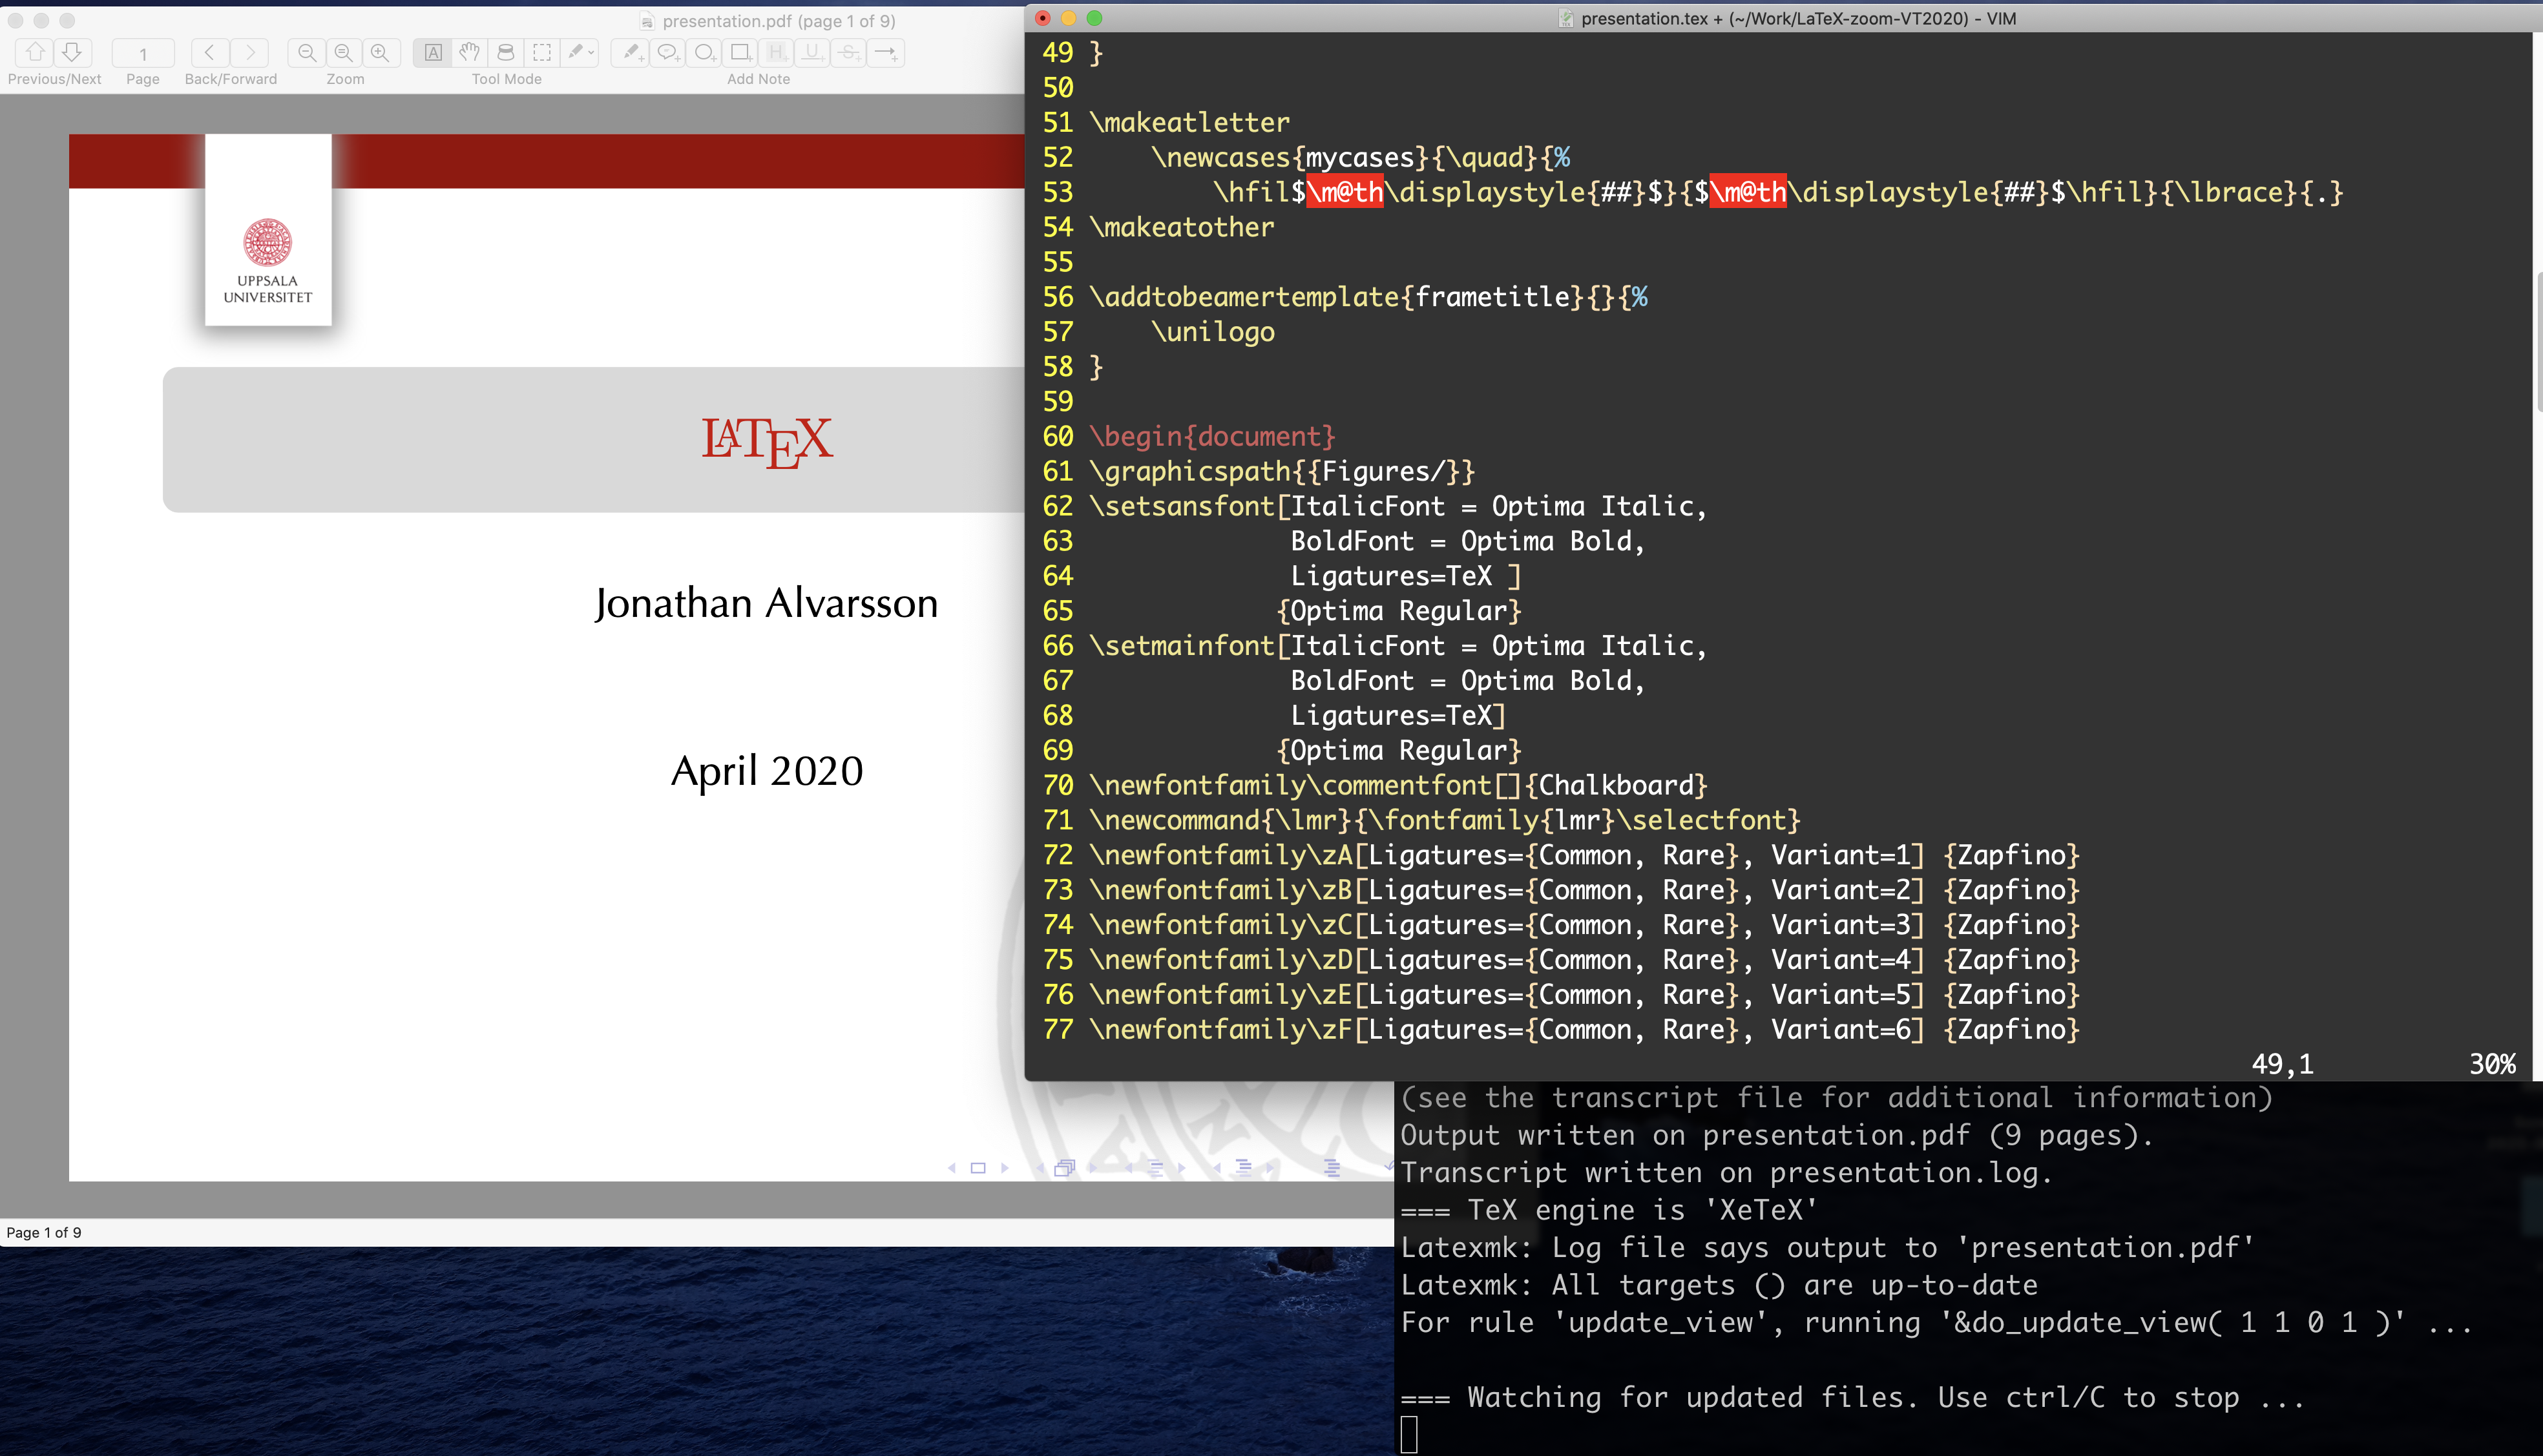
\includegraphics[width=1\textwidth]{figures/vim.png}}
    \end{frame}
    \subsection{Texshop}
    \begin{frame}
        \frametitle{Texshop}
        \framesubtitle{Texshop is a Mac program for typesetting using {\lmr \LaTeX}}
        \fbox{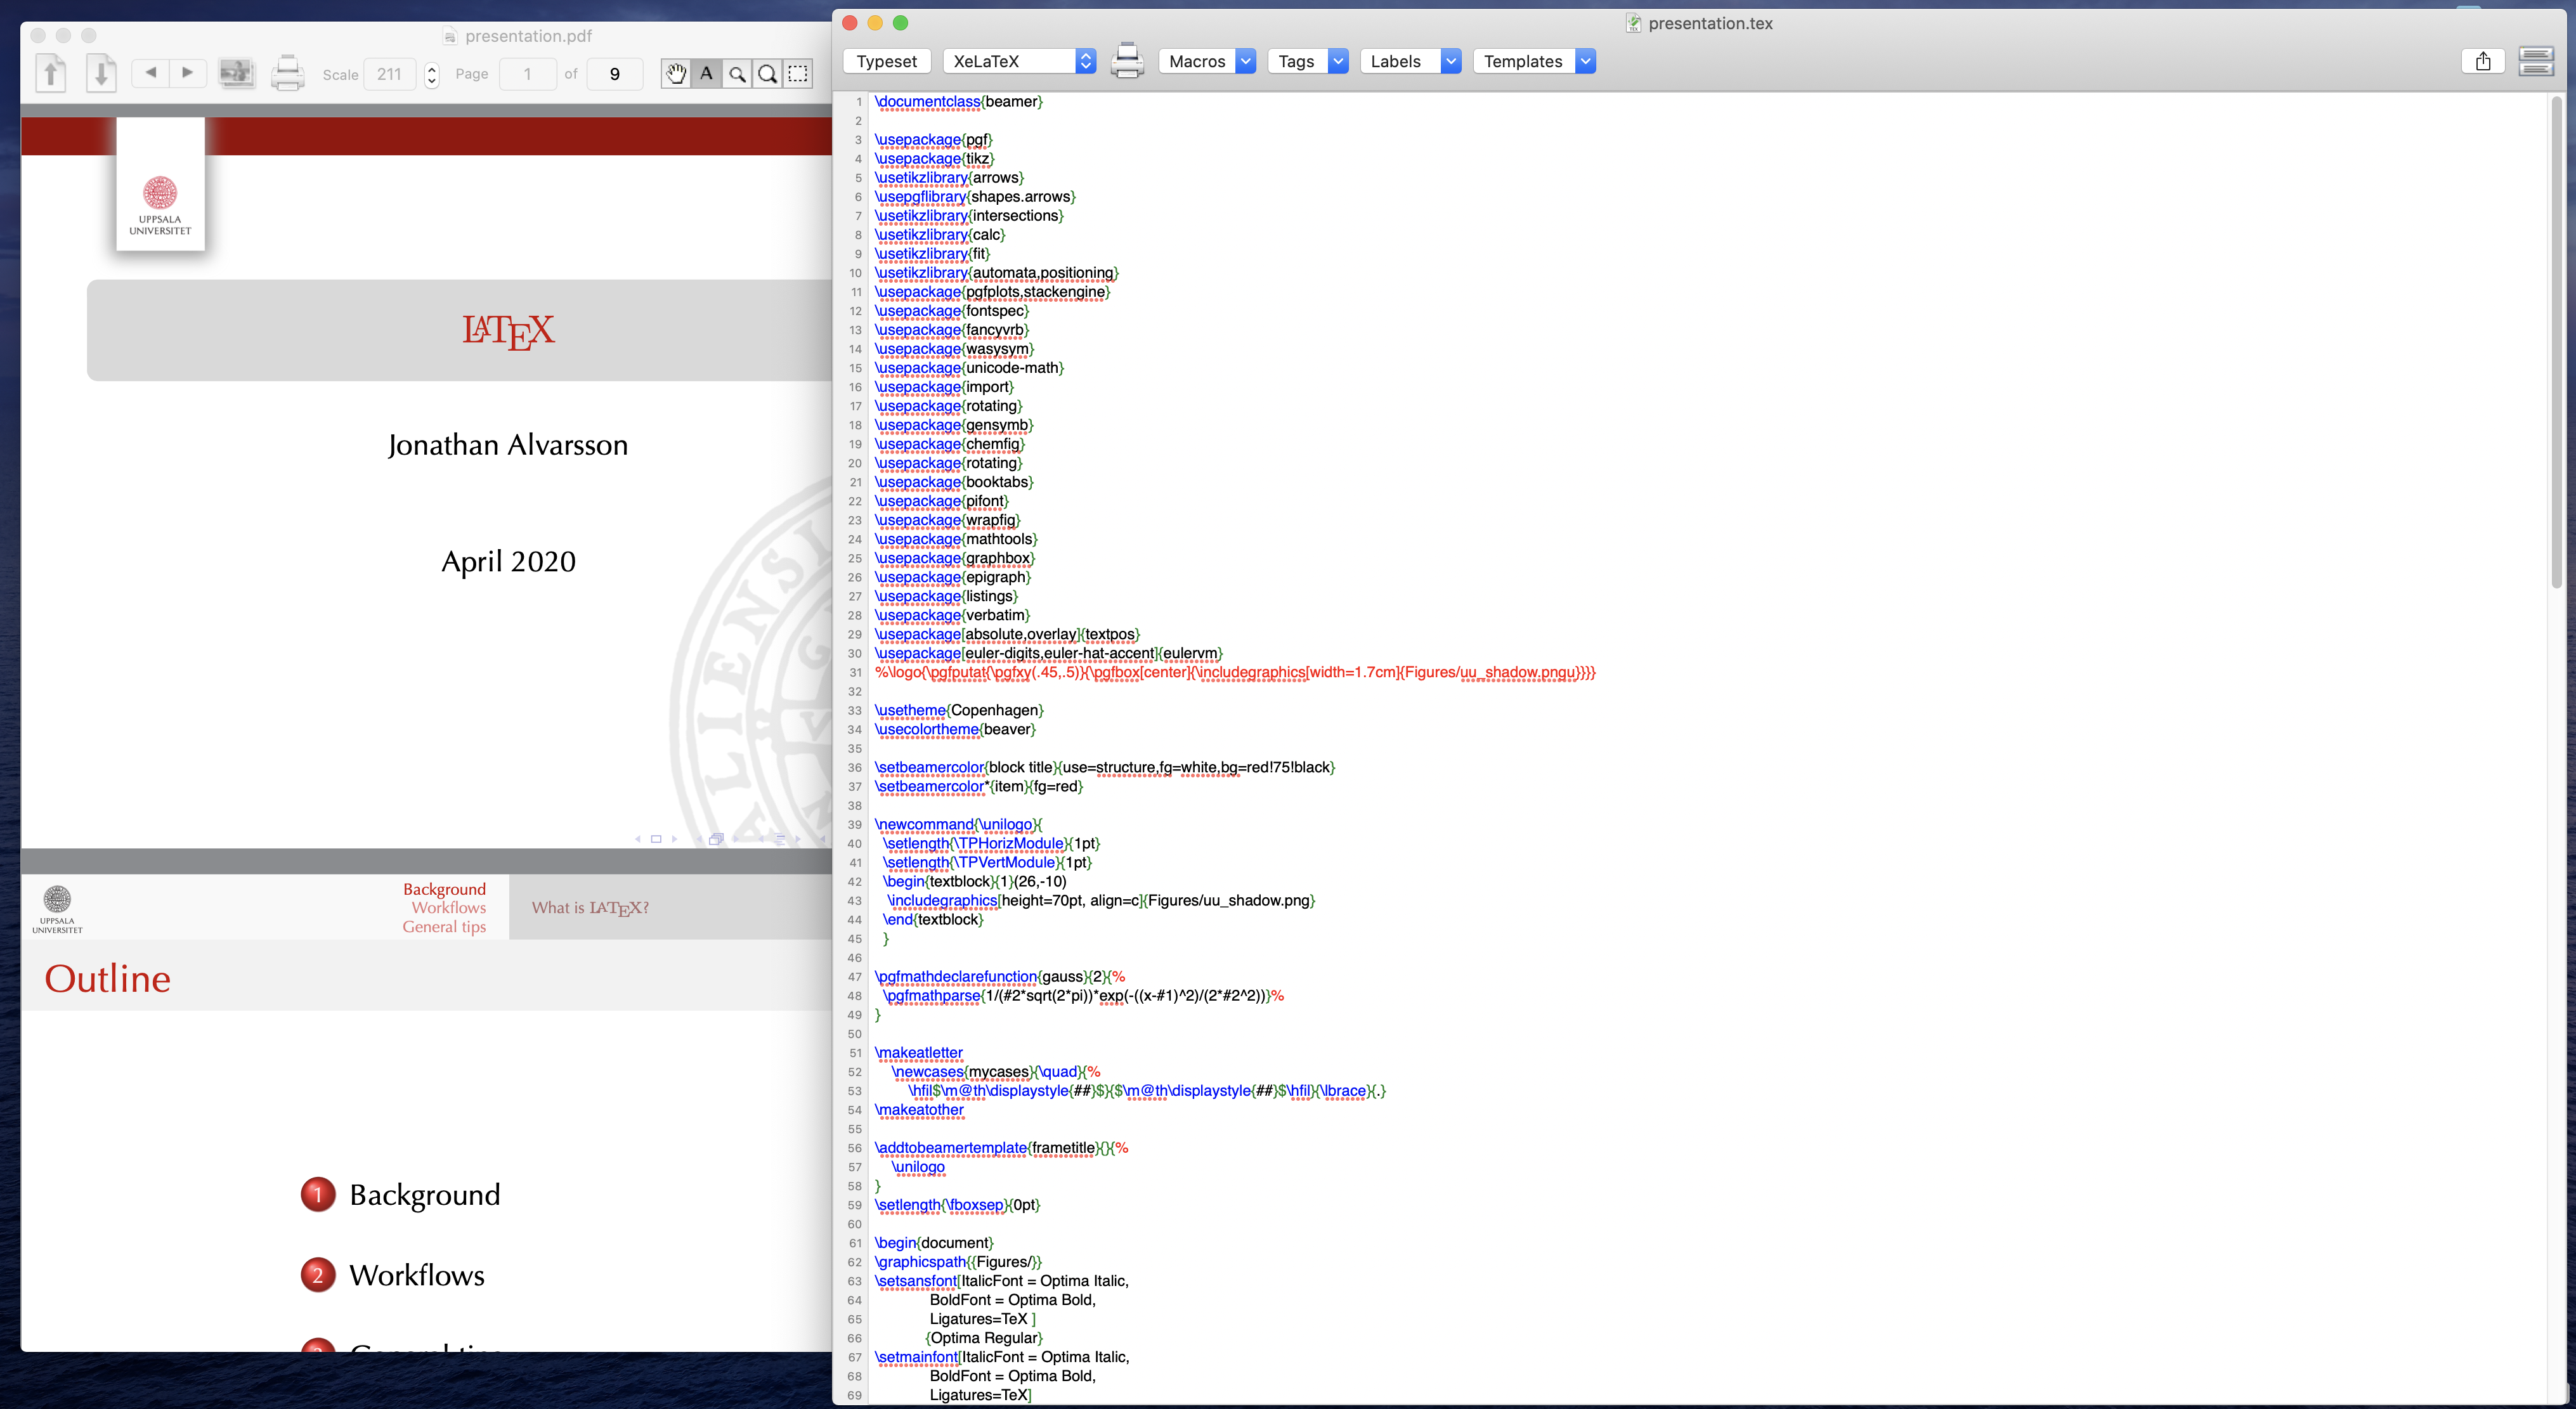
\includegraphics[width=1\textwidth]{figures/texshop.png}}
    \end{frame}
    \subsection{Overleaf}
    \begin{frame}
        \frametitle{Overleaf}
        \framesubtitle{Overleaf is an online solution with good and bad things}
        \centering
        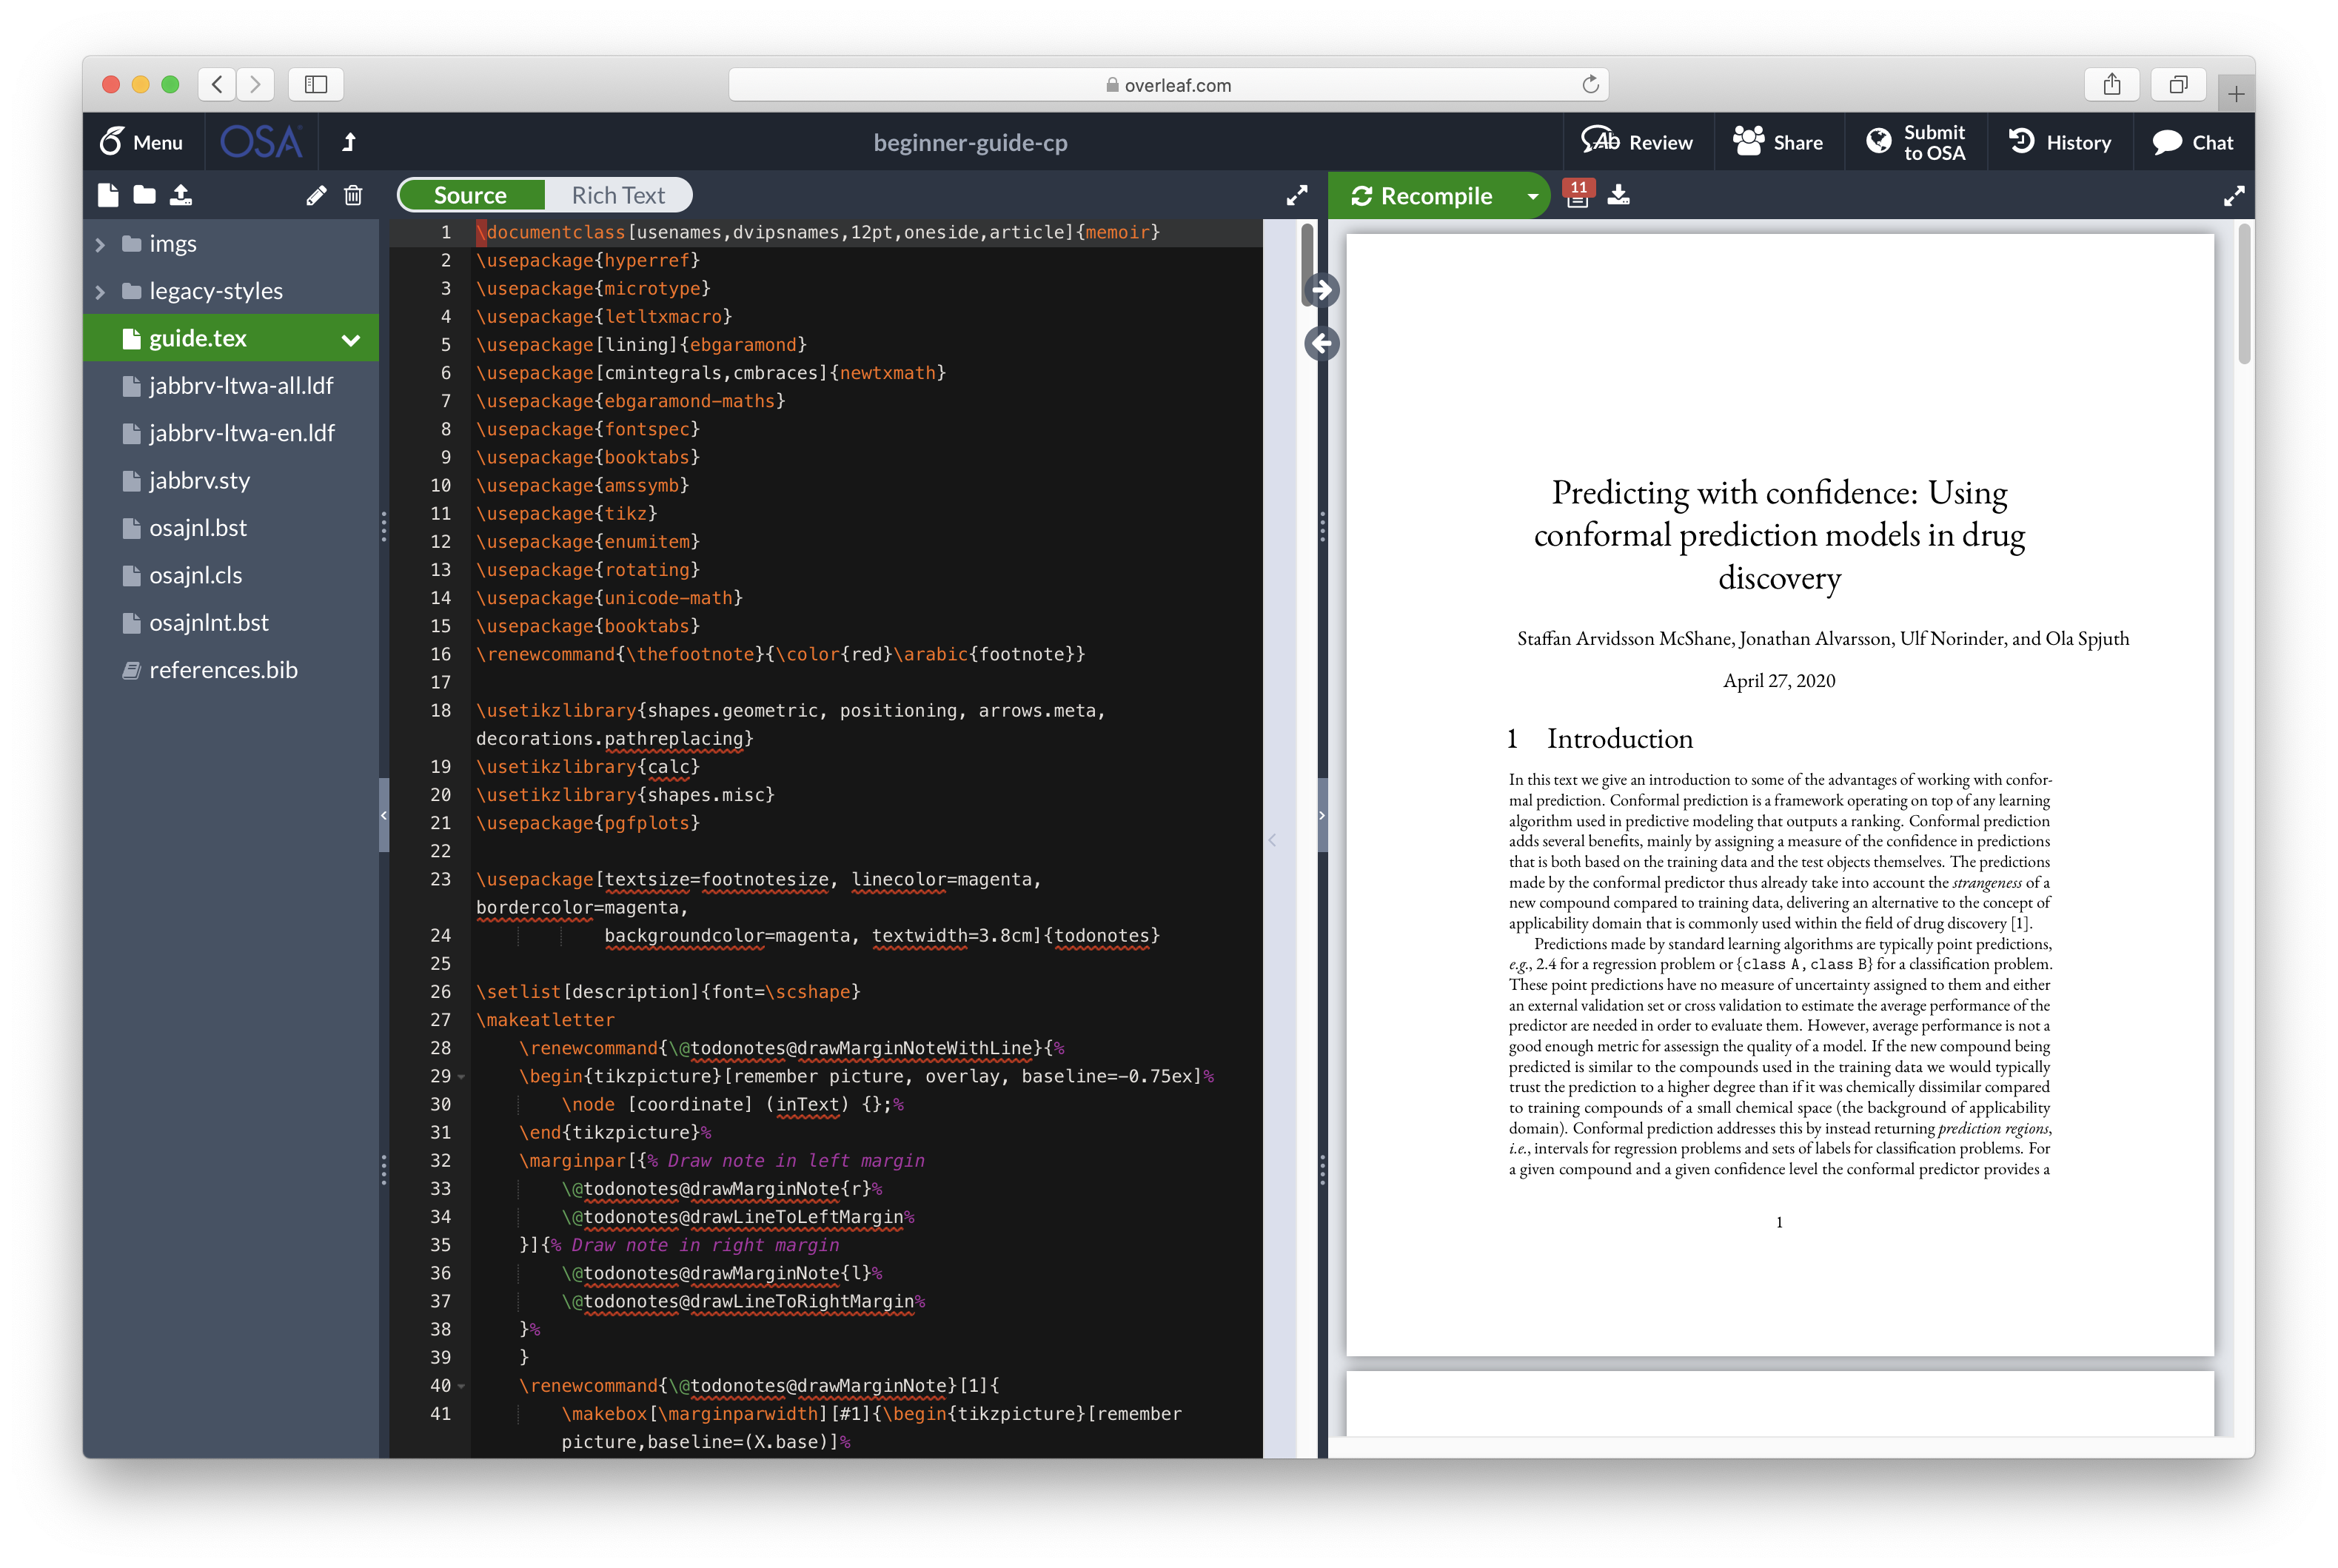
\includegraphics[width=0.95\textwidth]{figures/overleaf.png}
    \end{frame}
    \section{General tips}
        \subsection{Document classes}
            \begin{frame}
                \frametitle{Document classes}
                \framesubtitle{}
                \begin{block}{Document classes}
                    Layout structure is specified by giving a document classes. Some common classes include:

                    \begin{center}
                    \begin{tabular}{ll}
                    \toprule
                        Document class & Used for \\
                        \midrule
                        article & for articles \\
                        letter & for letters \\
                        book & for books \\
                        beamer & for presentations (like this one) \\
                    \bottomrule
                    \end{tabular}
                    \end{center}
                \end{block}
            \end{frame}
            \begin{frame}
                \frametitle{Document classes}
                \framesubtitle{}
                \begin{block}{Document classes}
                    However if you are writing something that will be printed
                    on paper \alert{I would recommend that you look at the
                    Memoir}\footnotemark
                    class. It has settings for anyting from article to book and
                    is very nice to work with!
                \end{block}
                \footnotetext{\scriptsize \mbox{Manual (615 pages) is at:
                    \url{http://texdoc.net/texmf-dist/doc/latex/memoir/memman.pdf}}}
            \end{frame}
        \subsection{Floats}
            \begin{frame}[fragile]
                \frametitle{Floats}
                \framesubtitle{Many people have a bit of a love/hate relationship with floats}
                \begin{block}{Floats}
                    The often used constructs \alert{figure and table creates floats}. 

                    For example, a figure is created like so:
                    
                    \begin{center}
                    \begin{minipage}{0.9\textwidth}
                    \begin{lstlisting}
\begin{figure}[htbp]
    \includegraphics[width=1\textwidth]{figs/myfig.png}
    \caption{My nice figure}
\end{figure}
                    \end{lstlisting}
                    \end{minipage}
                    \end{center}
                \end{block}
            \end{frame}
            \begin{frame}
                \frametitle{Floats}
                \framesubtitle{Many people have a bit of a love/hate relationship with floats}
                \begin{block}{Floats}\small
                    Floats can `float' in the text and be placed automagicly in
                    a good spot. \uncover<2->{This does not always work the way you expect
                    but it is possible to give it some instructions:
                    \begin{center}
                    \begin{tabular}{cp{0.6\textwidth}}
                    \toprule
                    Instruction & Meaning \\
                    \midrule
                    h & Place it here (kinda, if it looks OK) \\
                    b & Place it at the bottom of a page \\
                    t & Place it at the top of a page \\
                    p & Place it on a page of it's own, possible together with other floats \\
                    \bottomrule
                    \end{tabular}
                    \end{center}}
                    \uncover<3->{You can also modify these instructions with an
                    `!' which sort of means ``I really want you to follow my
                    instructions \uncover<4->{(but only if it doesn't look too bad (of
                    course))''}}
                \end{block}
            \end{frame}
            \begin{frame}[fragile]
                \frametitle{Floats}
                \framesubtitle{Many people have a bit of a love/hate relationship with floats}
                \begin{block}{Floats}
                    If you find yourself writing something like
                    \begin{center}
                    \begin{minipage}{0.9\textwidth}
\begin{lstlisting}
    \begin{figure}[!h]
    ...
\end{lstlisting}
                    \end{minipage}
                    \end{center}
                    and then crying a bit because the compiler doesn't care
                    about your \texttt{!h} instruction then that is because
                    putting a float there actually does not look good. However
                    if you still want to do it let me teach you a trick\ldots\ 
                        {\DejaSans ☺} 
                \end{block}
            \end{frame}
            \begin{frame}[fragile]
                \frametitle{Floats}
                \framesubtitle{Many people have a bit of a love/hate relationship with floats}
                \begin{block}{Floats}
                If you use the \texttt{float} package you can give the
                instruction \texttt{H} which turns of the floating all
                together. So it is a handy way of creating, \textit{e.g.}, a
                figure that looks like a proper figure but does not float. 
                \begin{center}
                    \begin{minipage}{0.9\textwidth}
\begin{lstlisting}
...
\usepackage{float}
...
\begin{figure}[H]
    \includegraphics[width=1\textwidth]{figs/myfig.png}
    \caption{My nice figure}
\end{figure}
\end{lstlisting}
                    \end{minipage}
                    \end{center}
                \end{block}
            \end{frame}

            \begin{frame}
                \frametitle{Floats}
                \framesubtitle{Many people have a bit of a love/hate relationship with floats}
                \centering
                While we are on the topic of floats\ldots
            \end{frame}

            \begin{frame}
                \frametitle{Floats}
                \framesubtitle{Many people have a bit of a love/hate relationship with floats}
                \begin{block}{Floats -- some more things}
                I thought I should also mention that (given that you use \texttt{Memoir} or the right packages) you:
                \begin{itemize}
                    \item can use a \texttt{\textbackslash FloatBlock} to make sure all floats are placed before a specific place in the text
                    \item are not limited to the predefined floats but can create your own floats (it is actually quite easy too) 
                \end{itemize}
                \end{block}
            \end{frame}

        \subsection{Small things}
            \begin{frame}
                \frametitle{Small things}
                \framesubtitle{Writing numbers}
                \begin{block}{Writing numbers}
                
                When you are writing numbers don't write them like:
                \begin{center}
                \begin{tabular}{rl}
                \toprule
                Example & Problem \\
                \midrule
                1000000 & unreadable  \\
                1,000,000 & confusing \\
                1.000.000 & confusing \\
                1 000 000 & too much space \\
                \bottomrule
                \end{tabular}
                \end{center}
                \end{block}
            \end{frame}
            \begin{frame}
                \frametitle{Small things}
                \framesubtitle{Writing numbers}
                \begin{block}{Writing numbers}
                Write them like:
                \begin{center}
                \begin{tabular}{rl}
                \toprule
                Example & Code \\
                \midrule
                1\,000\,000 & \texttt{1\textbackslash,000\textbackslash,000} \\
                \bottomrule
                \end{tabular}
                \end{center}
                \end{block}
            \end{frame}

            \begin{frame}
                \frametitle{Small things}
                \framesubtitle{In figures and tables use \textbackslash centering}
                \centering
                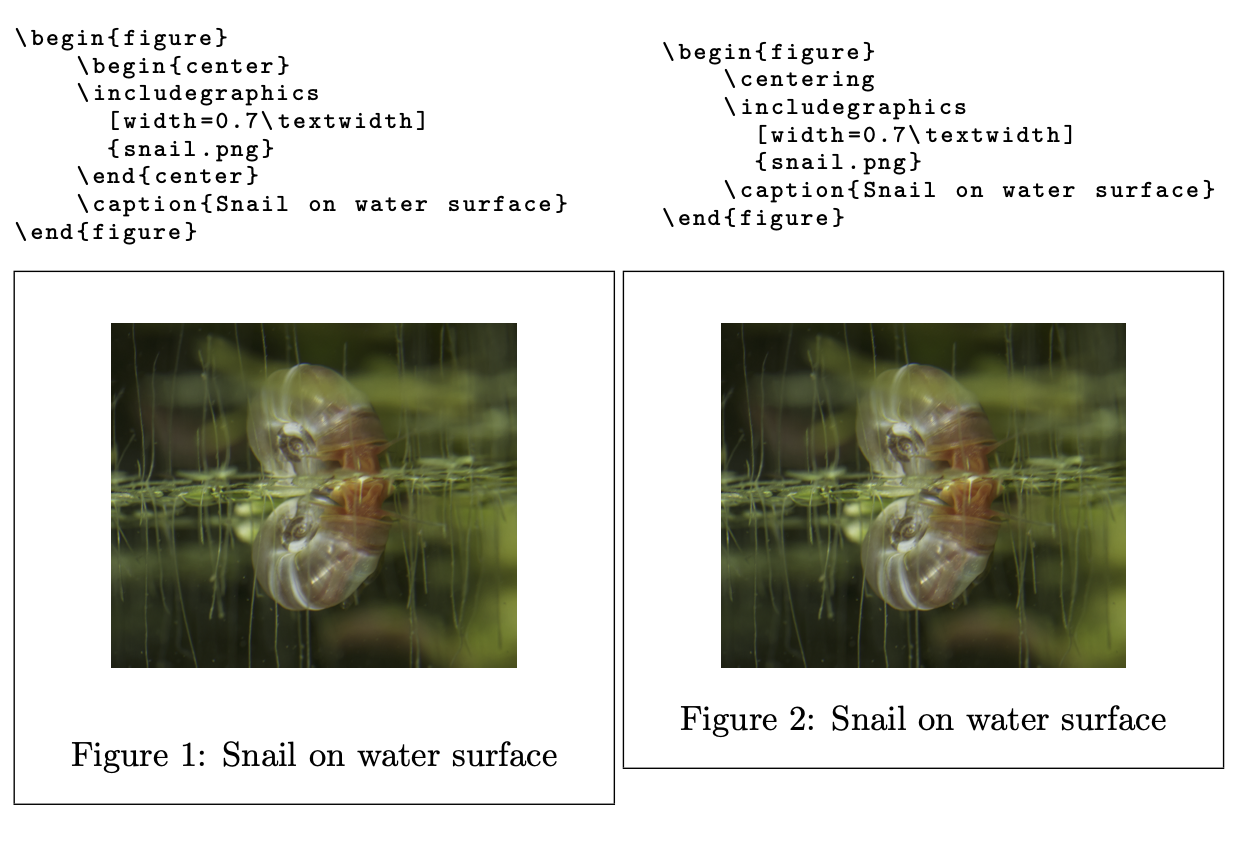
\includegraphics[width=0.9\textwidth]{figures/centering-example.png}
            \end{frame}
            
            \lstset{language=Tex, basicstyle=\ttfamily\tiny, frame=single }
            \begin{frame}[fragile]
                \frametitle{Small things}
                \framesubtitle{Non breaking space}
                \begin{block}{Use \texttt{$\sim$} for non breaking space.}
                \begin{minipage}{0.45\textwidth}
                    \centering
                    \begin{minipage}{0.95\textwidth}
                    \begin{lstlisting}
When writing things like 125 cm and
things like see Figure 2 it is nice
to keep things on the same line.
                    \end{lstlisting}
                    \end{minipage}
                \end{minipage}
                \hfill
                \begin{minipage}{0.45\textwidth}
                    \centering
                    \begin{minipage}{0.95\textwidth}
                    \begin{lstlisting}
When writing things like 125~cm and
things like see Figure~2 it is nice
to keep things on the same line.
                    \end{lstlisting}
                    \end{minipage}
                \end{minipage}

                \begin{minipage}{0.45\textwidth}
                When writing things like 125 cm and things like see
                Figure 2 it is nice to keep things on the same line.
                \end{minipage}
                \hfill
                \begin{minipage}{0.45\textwidth}
                When writing things like 125~cm and things like see
                Figure~2 it is nice to keep things on the same line.
                \end{minipage}
                \end{block}
            \end{frame}

            \begin{frame}
                \frametitle{Small things}
                \framesubtitle{Fonts}
                \begin{center}
                    Fonts is not really a ``Small things'' thing\ldots
                
                \uncover<2>{Nevertheless I am going to say something about it.}
                \end{center}
            \end{frame}

            \begin{frame}
                \frametitle{Small things}
                \framesubtitle{Fonts}
                Since {\lmr \LaTeX} is such an old thing the way we handle
                fonts has changed a bit since back then. The program we
                traditionally use (today) for compiling is called
                {\lmr\hologo{pdfLaTeX}} but there are at least two other
                programs that I can recommend {\lmr\hologo{LuaLaTeX}} and
                {\lmr\hologo{XeLaTeX}} which are capable of handling modern
                fonts directly. 
            \end{frame}
            
            \begin{frame}
                \frametitle{Small things}
                \framesubtitle{Fonts}
                \begin{block}{Fonts}
                Both {\lmr\hologo{LuaLaTeX}} and
                {\lmr\hologo{XeLaTeX}} use the \texttt{fontspec} package to specify fonts.  
                {\lmr\hologo{XeLaTeX}} is even able to handle the multiple
                glyphs found in the font:
                
                \centering
                {\zA Zapfino}
                \end{block}
            \end{frame}

            \frame[fragile=singleslide]{
                \frametitle{Small things}
                \framesubtitle{Fonts}
    Use the \texttt{fontspec} package to:
    \begin{block}{Set main font}
        \footnotesize 
        \Verb+\setmainfont[ItalicFont = Times New Roman Italic]{Times New Roman}+   

        {\timesfont To change the main font in your text, including \textit{italics}.}
    \end{block}
    \centering or
    \begin{block}{Create a toggle font command}
        \Verb+\newfontfamily\herculanum{Herculanum}+

        {\herculanum To, for example, use a crazy font in shorter parts.}
    \end{block}
}
            
            \appendix
            \section{Questions?}
            \subsection{Questions for me?}
            \begin{frame}
                \frametitle{Questions?}
                \framesubtitle{Questions for me?}
               \centering
               \Large Any questions? 

               \uncover<2>{If I can't answer there is always\ldots}
            \end{frame}

            \subsection{\{{\lmr \TeX}\}}
            \begin{frame}
                \frametitle{Questions?}
                  \begin{textblock}{1}(0,3)
                     
\includegraphics[width=1\paperwidth, align=c]{Figures/stackexchange.png}
                  \end{textblock}
                  \centering
                \Large \url{https://tex.stackexchange.com/}
            \end{frame}

    \setbeamertemplate{background}{%
        \parbox[c][\paperheight]{\paperwidth}{%
            \vskip -14 ex \hskip -5 em
            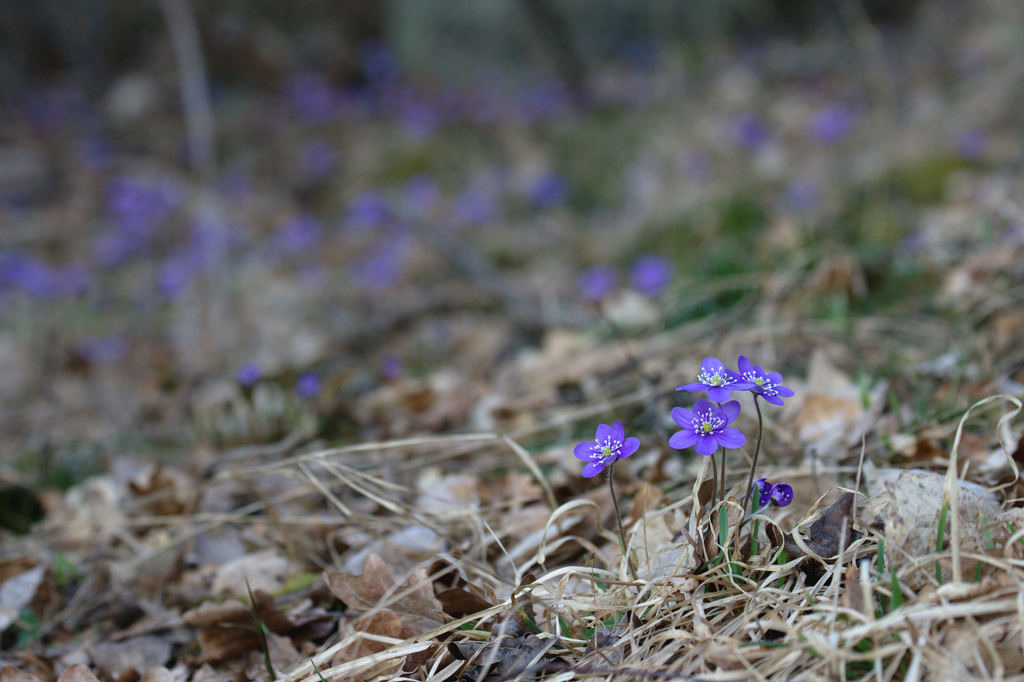
\includegraphics[height=1.275\paperheight]{Figures/blasippa.jpg}
        }   
    }
    \begin{frame}[plain]
        \vfill{\Huge\qquad\color{white} \zB Thank \zC you}\vfill
    \end{frame}
    \setbeamertemplate{background}{}
\end{document}
